
\medskip

\hrulefill\par
\href{https://manuel.sesamath.net/numerique/diapo.php?atome=48740&ordre=1}{\textcolor{blue}{\underline{\textit{Source : Manuel Sésamath 3e sous licence GnuFDL 1.1}}}}
\par\hrulefill
\medskip

Une famille se promène au bord d'une rivière.

Les enfants aimeraient connaître la largeur de cette rivière.

Ils prennent des repères, comptent leurs pas et dessinent le schéma ci-dessous sur lequel les points $C$, $E$ et $D$, de même que $A$, $E$ et $B$ sont alignées. (Le schéma n'est pas à l'échelle).

\begin{center}
%  \begin{tikzpicture}
%    \coordinate[label=below left:$A$] (A) at (0, 0);
%    \coordinate[label=above right:$B$] (B) at (12, 0);
%    \coordinate[label=below right:$D$] (D) at (12, -2);
%    \coordinate[label=above:$C$] (C) at (0, 3);
%    \coordinate[label=below:$E$] (E) at (intersection of C--D and A--B);
%    \draw[thick] (C) -- (A) -- (E) node[below, midway] {\scriptsize $20$ pas}
%    -- (B) node[midway, above] {\scriptsize $5$ pas} -- (D)  node[midway, right] {\scriptsize $1$ pas}
%    -- (C);
%    \draw[thin] ($(A)+(0,0.3)$)-|($(A)+(0.3,0)$);
%    \draw[thin] ($(B)+(0,-0.3)$)-|($(B)+(-0.3,0)$);
%    \node[inner sep=8pt,draw, rounded corners] at (6,4) {$AE=20$ pas~;  $BE=5$ pas~;  $BD=1$ pas};
%  \end{tikzpicture}
%\includegraphics[scale=0.7]{arbres.eps}
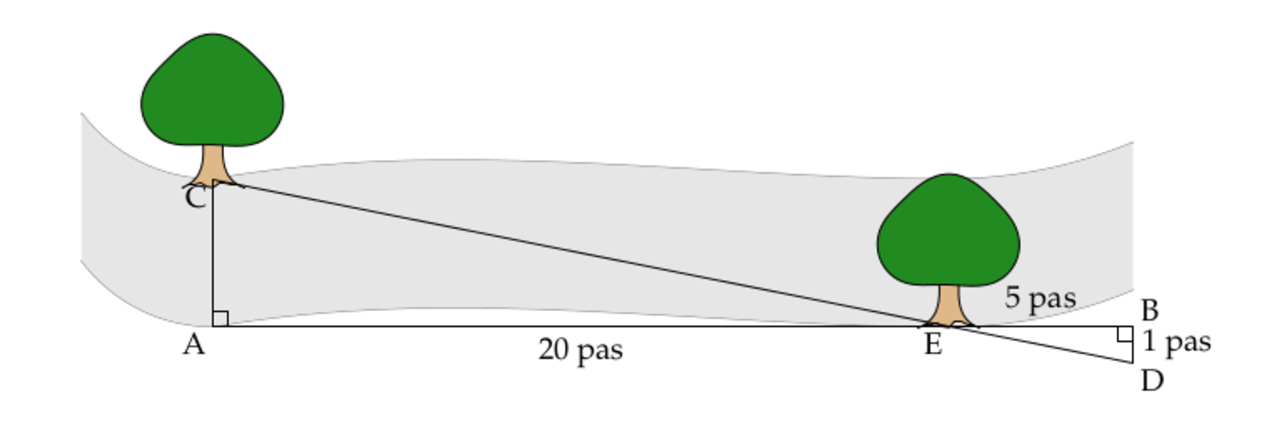
\includegraphics[scale=0.7]{arbresCP.eps}
\par\vspace{0.25cm}
\hrulefill\par
\textit{Illustration de Christophe Poulain}
\end{center}

\begin{enumerate}[itemsep=1em]
\item Démontrer que les droites $(AC)$ et $(BD)$ sont parallèles.
\item Déterminer, en nombre de pas, la largeur $AC$ de la rivière.
\end{enumerate}\medskip

Pour les questions qui suivent, on assimile la longueur d'un pas à $65\,\text{cm}$.
\begin{enumerate}
  \setcounter{enumi}{2}
\item Montrer que la longueur $CE$ vaut $13,3\,\text{m}$, en arrondissant au décimètre près.
\item L'un des enfants lâche un bâton dans la rivière au niveau du point $E$. Avec le courant, le bâton se déplace en ligne droite en 5 secondes jusqu'au point $C$.
  \begin{enumerate}
  \item Calculer la vitesse du bâton en m/s.
  \item Est-il vrai que \og{}Le bâton se déplace à une vitesse moyenne inférieure à $10\,\text{km/h}$\fg{}~?
  \end{enumerate}
\end{enumerate}
\medskip


